% !TEX root = ./main.tex
% ========================================================================== %
\section{Algorithm} \label{sec:algo}

The goal of \panco\ is to infer a measurement of a pressure profile and of its confidence intervals from the SZ map of a cluster.
The overall workflow implemented in \panco\ to perform this measurement is presented in Figure~\ref{fig:workflow}.
It is based on the forward modeling of the SZ map and on Monte-Carlo Markov Chain (MCMC) sampling of the probability distribution for the pressure profile parameters given the input data.
In this section, we detail each step of the analysis, as well as the inputs to be given to \panco\ and the results it produces.

\begin{figure*}[htp]
    \centering
    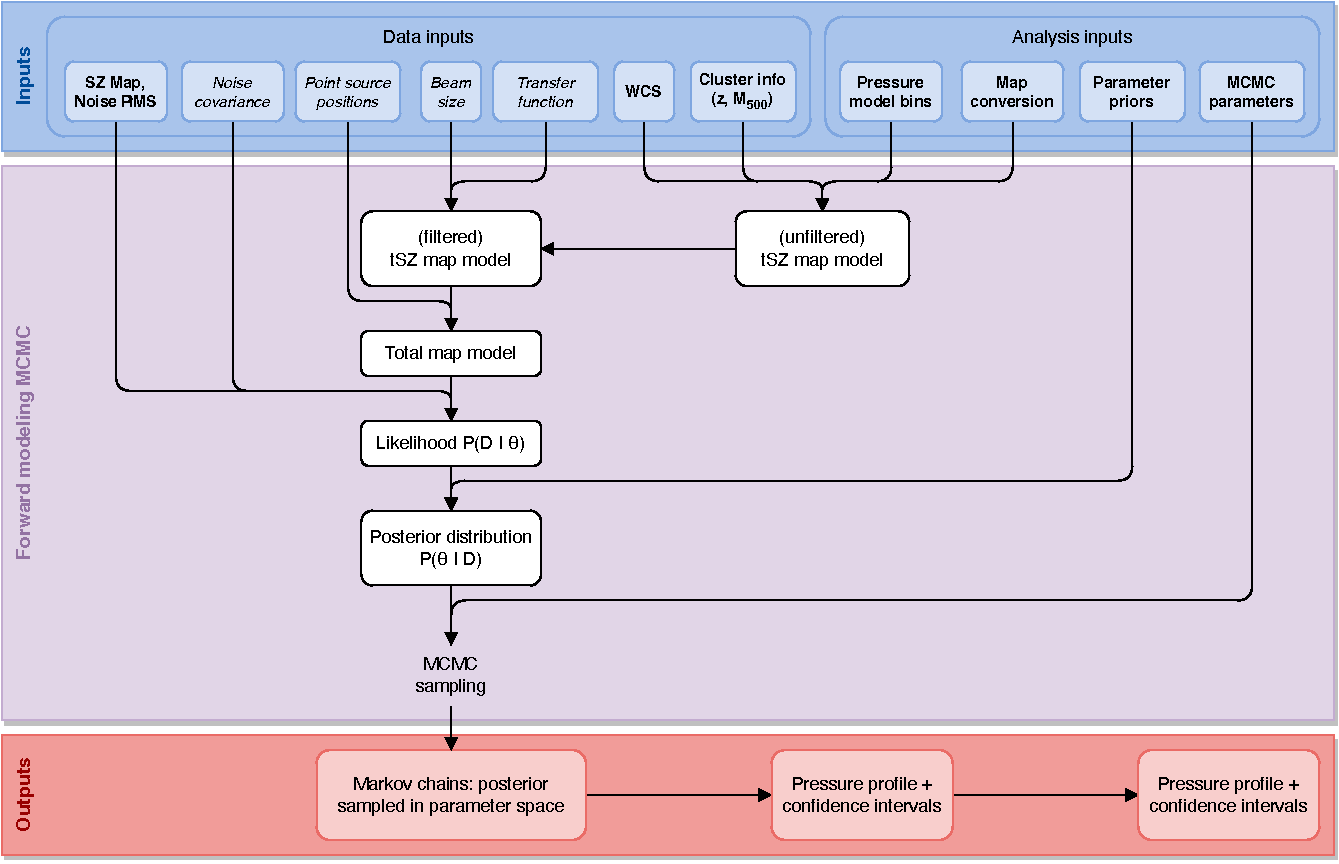
\includegraphics[width=.9\linewidth]{Figures/workflow.drawio.pdf}
    \caption{
        Schematic workflow of the \panco\ algorithm, from its inputs (blue), to the forward modeling and MCMC sampling (purple), and results (red).
        Required and optional inputs are denoted with boldface and italic fonts, respectively.
    }
    \label{fig:workflow}
\end{figure*}

% -------------------------------------------------------------------------- %
\subsection{Data inputs} \label{sec:algo:inputs}

The main input of \panco\ is a mapping of a patch of the sky containing SZ signal.
The code uses the FITS standard \citep{wells_fits_1981} to correctly map sky coordinates to pixels using the flat-sky approximation.
The map to be fitted must therefore be contained within a FITS file, that must include the following ingredients:

\begin{itemize}[leftmargin=*]
    \item An extension in which the data is the SZ map to be fitted, and the header includes the World Coordinate System (WCS) used to create the map;
    \item An extension in which the data represent an estimate of the expected root mean squared (RMS) error for each pixel of the data map.
\end{itemize}

Such a file constitutes the minimum data input for \panco\ to proceed fitting a pressure profile.
Using these inputs, the user may choose to only use a square portion of the map, by specifying the sky coordinates of its center and its side.

Additional inputs can be provided to account for various data features.
\paragraph{Beam smearing} the user may provide the width of a Gaussian function to account for point spread function (PSF, hereafter referred to as ``beam'') filtering (see \S\ref{sec:algo:fwdmod});
\paragraph{Transfer function} Fourier filtering due to data processing and/or scanning strategy can be accounted for in the analysis (see \S\ref{sec:algo:fwdmod});
\paragraph{Point source contamination} the position on the sky of point sources, as well as their fluxes and uncertainties, can be used to account for the contamination and marginalize over its amplitude (see \S\ref{sec:algo:fwdmod});
\paragraph{Correlated noise} the covariance matrix between the noise of pixels in the map can be provided (see \S\ref{sec:algo:likelihood});
\paragraph{Integrated SZ signal} an external measurement of the integrated Compton parameter, that may be used as a constraint on large-scale tSZ signal, can be given to \panco\ (see \S\ref{sec:algo:likelihood}).

% -------------------------------------------------------------------------- %
\subsection{Pressure profile model} \label{sec:algo:press}

The electron pressure distribution in the ICM is modeled in \panco\ as a radial pressure profile, implying spherical symmetry of the ICM.
The most widely used parametrization for ICM pressure profiles, called the generalized Navarro-Frenk-White model \citep[gNFW,][]{zhao_analytical_1996, nagai_effects_2007}, is known to have several shortcomings.
In particular, the very self-constrained shape of the functional form of the profile and the important correlations in the parameter space make model fitting complex, and the recovered parameter values hard to interpret \citep[see \eg][]{nagai_effects_2007, battaglia_cluster_2012-1, sayers_evolution_2022}.

In order to try to circumvent these issues, \panco\ uses a more flexible parametrization of the pressure profile, in which the pressure distribution is modeled as a power law evolution in concentric spherical shells.
In this modeling, the model parameters are the values $P_i$ of the pressure profile at predefined radii from the cluster center $R_i$, with a power law interpolation between the radii\footnote{Several papers in the literature have dubbed this modeling a ``non-parametric'' approach; as this may induce confusion, since the model is parametric, we will refrain from using this term, and refer to our model as ``radially binned''.}:
\begin{equation}
    \label{eq:algo:pressure_profile}
    P(r \in [R_i, R_{i+1}[) = P_i \left(r / R_i\right)^{-\alpha_i},
\end{equation}
where $\alpha_i = - \log(P_{i+1} / P_i) / \log(R_{i+1} / R_i)$. \\
Outside of the radial bins, the pressure profile is extrapolated using the power-law evolution of the first (last) bin.
In addition to being more flexible and having generally lesser correlations in the parameter space, this parametrization can be integrated along a line of sight analytically through Abell transform, by following \eg\ \citet{romero_multi-instrument_2018}.

The main downside to this pressure profile modeling lies in the need to specify the radii $R_i$ used in \refeq{eq:algo:pressure_profile} \textit{a priori} when performing a fit.
There is no obvious, fail-safe way to define this radial binning.
A user may choose a binning motivated by the data coverage (\eg\ with radii that, projected on the sky plane, are separated the beam of the instrument used to build the map); but looking at the same data, another user may be motivated by sample studies over several cluster, and wish to define a binning in units of a characteristic radius of the cluster (\eg\ $R_{500}$).
As a result, model dependence may arise in the results produced by \panco.
This point will be addressed in \S\ref{sec:end}.

% -------------------------------------------------------------------------- %
\subsection{Forward modeling: from pressure profile to SZ map} \label{sec:algo:fwdmod}

\begin{figure}
    \centering
    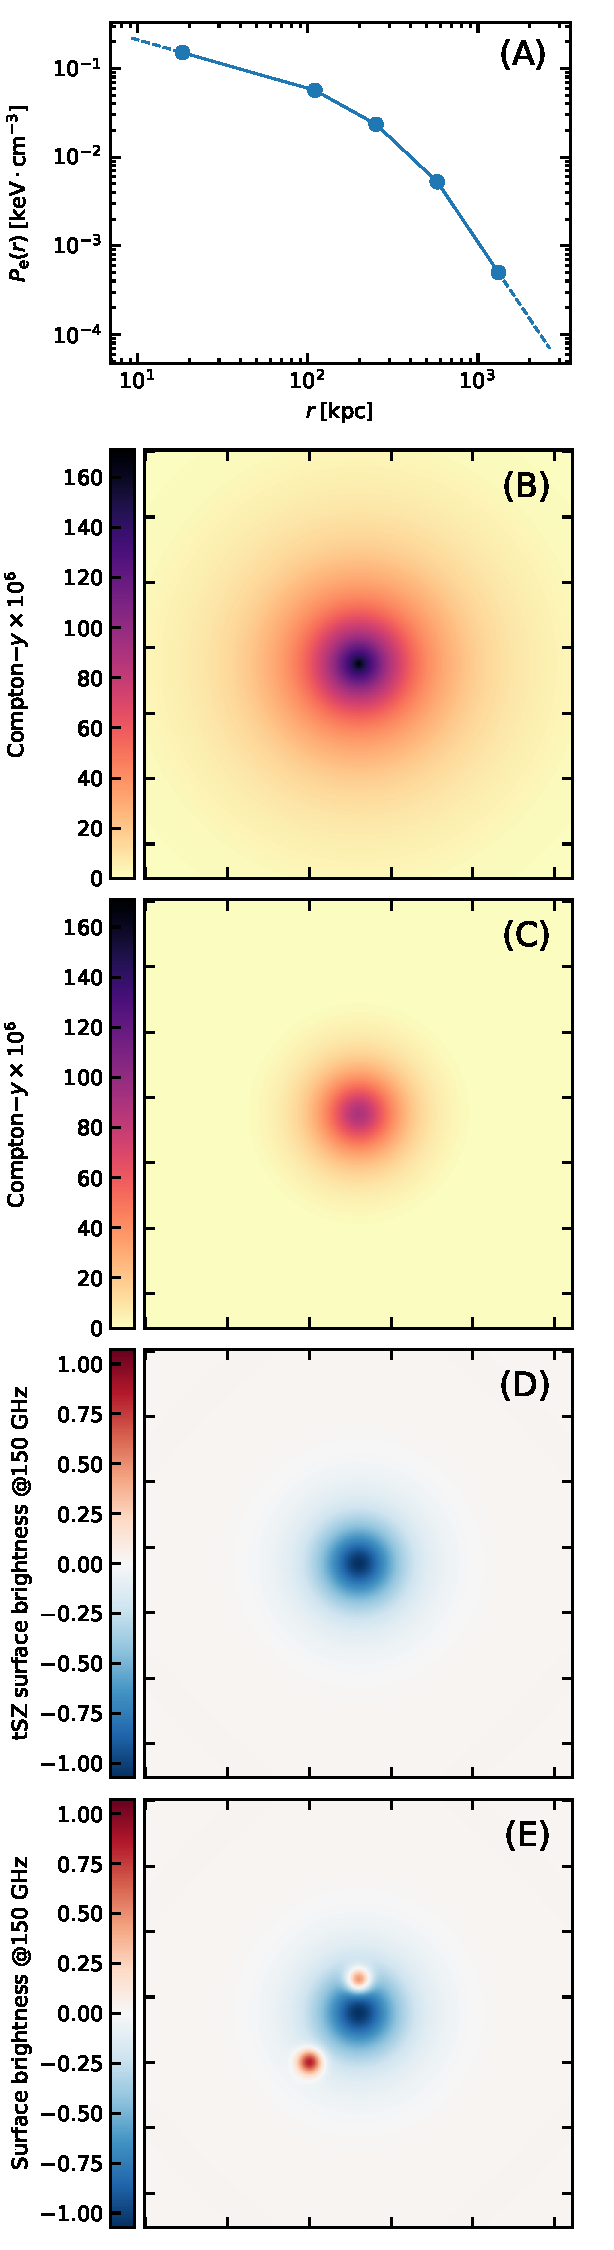
\includegraphics[height=0.933\textheight]{Figures/fwmod.pdf}
    \caption{
        Illustration of the forward modeling procedure.
        The pressure profile (A) is integrated along the line of sight to create a Compton$-y$ map (B), which is filtered (C) and converted (D) to be realistically comparable to the observed data.
        If point source contamination information is passed, point source models can be added to the map (E).
    }
    \label{fig:fwmod}
\end{figure}

The approach used by \panco\ to fit pressure profiles on SZ maps is forward modeling.
In that framework, a pressure profile model -- determined by \refeq{eq:algo:pressure_profile} -- is used to generate a map that can be compared to data.
This approach has been vastly used in the estimation of pressure profiles from tSZ maps, especially in the context of resolved follow-up of galaxy clusters with \eg\ NIKA2 \citep[\eg][]{munoz-echeverria_multi-probe_2022,keruzore_exploiting_2020}, MUSTANG(2) \citep[\eg][]{romero_galaxy_2017,romero_pressure_2020}, Bolocam \citep[\eg][]{sayers_evolution_2022}, or ALMA \citep[\eg][]{di_mascolo_joint_2019}.
This section details the different steps used in that process, which is ilustrated in figure~\ref{fig:fwmod}.

\paragraph{Line of sight integration}

The amplitude of the tSZ effect in a direction $\theta$ on the sky is named the Compton parameter $y$, and is proportional to the integral along of the electron pressure along the line of sight (LoS):
\begin{equation}
    \label{eq:algo_ysz}
    y(\theta) = \frac{\sigma_\textsc{t}}{m_{\rm e}c^2} \int_{\rm LoS(\theta)} P_{\rm e} \; \dd l,
\end{equation}
where $\sigma_\textsc{t}$ is the Thompson cross-section, and $m_{\rm e} c^2$ is the electron resting energy. \\
In \panco, we perform this integration analytically, by following the derivation presented in Appendix A of \citet{romero_multi-instrument_2018}, using the spherically symmetric case (in the notation of \citeauthor{romero_multi-instrument_2018}, $a_i = b_i = c_i = 1 \; \forall \; i$).
This allows us, for any given pressure profile, to create a Compton parameter map in the same coordinate system as the data, \ie\ an estimate of the value of $y$ for each pixel in the map.

\paragraph{Conversion and zero level}

Depending on the data product available, and on the convention used in the raw data processing software employed to create these data products, tSZ maps can have a variety of units (\eg\ surface brightness, CMB temperature fluctuation).
These units can usually be converted to Compton$-y$ through a scalar conversion coefficient, $C_{\rm conv}$, which can depend on many different quantities that may be difficult to estimate, or even fluctuate during observations, such as instrumental bandpasses, weather conditions, instrumental calibration, or even temperature of the ICM through relativistic corrections to the tSZ effect \citep{mroczkowski_astrophysics_2019}.
As a result, the conversion coefficient is affected by an uncertainty.
In \panco, this coefficient is treated as a parameter in the model, for which a prior distribution needs to be specified (see \S\ref{sec:algo:mcmc}), allowing to propagate the uncertainty on the conversion of the map to the pressure profile estimate.
This means that a vector in the parameter space will contain a value of a conversion coefficient, which \panco\ multiplies the model $y-$map by to get a map in the same units as the input data.
In case the input data is already in units of Compton$-y$, this coefficient may still be used to propagate multiplicative calibration uncertainty by centering the prior distribution on 1.
In addition, in order to enable taking into account possible large-scale residual noise, a zero-level offset can be added to the map, and marginalized over.

\paragraph{Filtering}

The tSZ maps constructed by any instrument are affected by different types of filtering.
The instrumental PSF acts as a filter that smooths the data by suppressing signal at small scales.
In its forward modeling approach, \panco\ is able to take into account this filtering by convolving the model $y-$map with a 2D Gaussian filter, the width of which can be specified by the user.

In addition, during the data reduction process used to create tSZ maps from raw data, filtering can occur, often suppressing signal at large angular scales.
This filtering is usually accounted for through a transfer function, quantifying the signal filtering in the Fourier space, and evaluated during the data processing.
\panco\ can account for this effect by filtering the map with a transfer function provided by the user.
Two different types of transfer functions can be provided:
\begin{itemize}[leftmargin=*]
    \item a 1D transfer function: assuming that the filtering is isotropic, \panco\ can convolve model maps with a 1D kernel specified by the user as angular frequencies $k$ and their associated filtering ${\rm TF}(k)$;
    \item a 2D transfer function: if the filtering on the sky cannot be assumed to be isotropic, the user may specify 2D angular scales $(k_x, k_y)$ and their corresponding filter ${\rm TF}(k_x, k_y)$.
\end{itemize}
A thorough discussion of the impact of choosing a 1D or 2D transfer function -- in the case of NIKA2 data, in which the filtering is mildly anisotropic -- can be found in \citet{munoz-echeverria_multi-probe_2022}.

\paragraph{Point source contamination}

After applying the different filters, the \panco\ model map is a map of the tSZ signal, in the unit and mapping as the input data, and having been affected by the same signal filtering.
It is therefore comparable to the tSZ signal in the input map.
But millimeter-wave maps of cluster regions may also include astrophysical signal from other sources.
In particular, signal from millimeter-emitting galaxies can often be found in such maps.
These galaxies can be foreground, background, or cluster members, and their emission can be thermal (in the case of dusty star-forming galaxies), or synchrotron (for radio-loud AGN).
In any case, this signal manifests as a contamination for tSZ science, and must be accounted for in data analysis, lest the recovered pressure profile be biased.

In its forward modeling approach, \panco\ uses the methodology described in \eg\ \citet{keruzore_exploiting_2020}, in which point source models may be added to the tSZ model map in order to model the total signal in the map.
The spatial model of each source is given by the instrumental PSF, and their fluxes are treated as model parameters, with priors specified by the user (see \S\ref{sec:algo:mcmc}).
If the flux of a source is well known from external data, this prior will be tight, and serve as a propagation of its uncertainty to the recovered pressure profile.
Otherwise, if a source is known to be present but little is known about its flux, large priors can be used, in which case \panco\ will constrain the sum of the tSZ signal and the point source flux\footnote{\panco\ is able to constrain the sum of the two because of the different spatial distribution of the tSZ and point source fluxes.}.
To account for point source contamination in the analysis, the user must therefore provide \panco\ with a position (in sky coordinates) and a probability distribution for the flux (in input map units) for each of the sources considered.

% -------------------------------------------------------------------------- %
\subsection{Likelihood} \label{sec:algo:likelihood}

The process described in \S\ref{sec:algo:fwdmod} allows \panco\ to compute a model map that is comparable to the input data from any position in the parameter space.
To summarize, a vector in this parameter space, $\vartheta$, has the following components:
\begin{itemize}[leftmargin=*]
    \item $P_0, \dots P_n$: the value of the pressure profile at each predefined radius $R_0, \dots R_n$ ; \\
    \item $C_{\rm conv}$: the conversion coefficient from Compton$-y$ to input map units;
    \item $Z$: a zero-level for the map;
    \item If provided, $F_0, \dots F_m$: the fluxes of point sources in the map, in input map units.
\end{itemize}

The comparison between the model map and the input data is performed through a Gaussian likelihood function:
\begin{align}
    \nonumber -2 \log \mathcal{L}(\vartheta) & \equiv -2 \log p(D | \vartheta) + {\rm cst.} \\
        & = \left[D - M(\vartheta)\right]^{\rm T} \mathbf{C}^{-1} \left[D - M(\vartheta)\right],
    \label{eq:algo:likelihood}
\end{align}
where $D$ is the input map, $M(\vartheta)$ is the model map computed from the position in parameter space $\vartheta$, and $\mathbf{C}$ is the noise covariance matrix. \\
If the noise in the map can be considered white, the noise values in the map pixels are uncorrelated, and $\mathbf{C}$ becomes diagonal.
In that case, in order to reduce the computation time needed, the likelihood is rewritten as:
\begin{equation}
    \label{eq:algo:likelihood_white}
    -2 \log \mathcal{L}(\vartheta) = \sum_i \left( \frac{D_i - M_i(\vartheta)}{\Sigma_i} \right)^2,
\end{equation}
where the sum runs over all pixels $i$ in the map, and $\Sigma$ is the noise RMS map.

In some cases, especially with high angular resolution follow-ups of clusters, additional information may be known from SZ surveys, such as the integrated tSZ signal $Y_{<R}$ within a radius $R$ of the cluster.
This knowledge can serve as an additional constraint on the model, by computing the value of the integrated tSZ signal from the model as the spherical integration of the pressure profile within the radius $R$.
This value can then be compared to that known from independent measurement, providing an additional data point that can be added to the log-likelihood of eqs.~(\ref{eq:algo:likelihood} or \ref{eq:algo:likelihood_white}):
\begin{equation}
    \label{eq:algo:likelihood_ysz}
    \left(\frac{Y_{<R}^{\rm meas.} - \frac{\sigma_\textsc{t}}{m_{\rm e}c^2}\int_{0}^{R} P_{\rm e}(r) \, r^2 \dd r}{\Delta Y_{<R}^{\rm meas.}} \right)^2,
\end{equation}
where $Y_{<R}^{\rm meas.}$ and $\Delta Y_{<R}^{\rm meas.}$ are the measured integrated SZ signal within $R$ and its uncertainty. \\
This additional constraint can be especially useful when dealing with observations agressively filtering large scale signal, in which case it might effectively provide constraining power on the pressure profile at large radii.
This approach is routinely used for NIKA2 tSZ follow-ups of SZ-detected clusters \citep[\eg][]{ruppin_first_2018,keruzore_exploiting_2020,munoz-echeverria_multi-probe_2022}.

% -------------------------------------------------------------------------- %
\subsection{Posterior distribution and MCMC sampling} \label{sec:algo:mcmc}

\panco\ performs the extraction of pressure profile from tSZ data using Bayesian MCMC.
In that framework, a prior probability distribution for the parameters, $p(\vartheta)$, must be multipled to the likelihood function of \refeq{eq:algo:likelihood} to obtain a posterior distribution for the parameters given the data: $p(\vartheta | D) \propto p(D | \vartheta) \, p(\vartheta)$.
In \panco, the prior distributions for the different model parameters are considered uncorrelated, meaning the prior distribution is the product of the individual priors on parameters:
\begin{equation}
    \label{}
    p(\vartheta) = \prod_i p(\vartheta_i),
\end{equation}
where the product runs over all individual parameters $i$. \\
The prior on each parameter is to be specified by the user, using the large variety of distributions available in the \texttt{scipy.stats}\footnote{\url{https://docs.scipy.org/doc/scipy/reference/stats.html}} module \citep{virtanen_scipy_2020}.

The resulting posterior distribution, $p(\vartheta | D)$, is then sampled using MCMC.
More specifically, we use the affine-invariant ensemble sampling implementation of the \texttt{emcee} library \cite{foreman-mackey_emcee_2019}.
Convergence of the walkers is monitored at regular intervals based on the autocorrelation length of the chains, using the following algorithm.
Every $n_{\rm check}$ steps (\ie\ accepted positions in the parameter space), the integrated autocorrelation length $\tau_j$ of each chain $j$ is computed, as well as the average autocorrelation over all chains, $\tau = \left< \tau_j \right>$.
Convergence is accepted if both of the two following criteria are met:
\begin{enumerate}[leftmargin=*]
    \item The current length of the chains is longer than $n_{\rm auto} \times \tau$;
    \item The mean autocorrelation has changed by less than $\Delta\tau_{\rm max}$ in the last two evaluations.
\end{enumerate}
The values of $n_{\rm auto}$ and $\Delta\tau_{\rm max}$ are parameters of \panco, that need to be specified by the user.
Likewise, the user needs to provide a maximum chain length at which the sampling should stop if convergence was never reached.

% -------------------------------------------------------------------------- %
\subsection{Chains cleaning and exploitation} \label{sec:algo:outputs}

Once MCMC convergence has been reached, \panco\ stores the full sampling of the posterior distribution, \ie\ all of the accepted positions in the parameter space and their associated log-likelihood and log-posterior values.
The raw chains can then be loaded and cleaned as follows:
\begin{enumerate}[leftmargin=*]
    \item Remove the first $n_{\rm burn}$ samples as a burn-in length;
    \item Thin the chains by discarding $(n_{\rm discard} - 1) / n_{\rm discard}$ samples, \ie\ only keeping one sample every $n_{\rm discard}$ steps;
    \item Discard the chains that are poorly mixed, \ie\ systematically outside of the $[q_{\rm extr}, 1 - q_{\rm extr}]$ quantiles of the sampled posterior.
\end{enumerate}
Again, the values of $n_{\rm burn}$, $n_{\rm discard}$ and $q_{\rm extr}$ are parameters of the analysis, that must be user-provided.

The cleaned chains can then be expressed in the pressure profile space.
To do so, \refeq{eq:algo:pressure_profile} is used to compute a profile for each position in the parameter space, over a radial range specified by the user.
These profiles may then be saved for future analyses.

The Markov chains, in the parameter space and in the pressure profile space, constitute the main data product of \panco.
Several figures can be produced for a visual representation of the results.
They are all presented in the technical documentation \todo{add link}; we give here a brief description of these figures.

\paragraph{Posterior distribution}
Several functions are available to produce figures showing properties of the Markov chains and the posterior distribution they sample, using the \texttt{ChainConsumer} library \citep{hinton_chainconsumer_2016}:
\begin{itemize}[leftmargin=*]
    \item Walks plot, \ie\ the evolution of the positions in the parameter space with the number of steps for each parameter;
    \item Corner plot, \ie\ a figure showing the marginalized posterior for all individual parameters and sets of two parameters.
        The prior distribution can be overplotted for comparison purposes;
    \item Plot of the correlation and covariance matrices of the different parameters.
\end{itemize}

\paragraph{Data -- Model -- Residuals}
Two figures can be produced to illustrate the quality of the fit.
They both consist in comparing the input data, the best-fitting model, and the residuals (\ie\ the difference between input data and best-fitting model).
These can be plotted in 2D, by showing the three maps side-by-side (see figure~\ref{fig:valid:dmr_2d}), or in 1D, by showing the radial profiles of each of these maps in the same graph (see the left panels of figure~\ref{fig:valid:profiles}).
Goodness of fit can be judged in both representations by lack of significant structure in the residuals.

\paragraph{Pressure profile}
In addition, a plot of the median of these profiles, as well as confidence intervals chosen as their 16th and 84th percentiles, can be produced (see the right panels of figure~\ref{fig:valid:profiles}).
